\chapter{Lecture six: OOA\&D in Practice}

\section{Software requirements}
\subsection{Unclear requirements}
There are many examples of problems with requirements. Unclear requirements have been denoted as the main source of problems in system development projects.

E.g: Amanda; the IT-system for Arbejdsformidlingen ended up costing 650+ million DKK, originally budgetted for 214 million DKK. It did not fit the work of the employees; for example, they had to go through 40-50 screens to register a single person as unemployed. The time spent per registration went from 10-20 minutes to one hour.

Examples of similar situations and causes of these:

\begin{itemize}
    \item Sundhed.dk; the information is flawed, it had been dropped, and rebudgeted multiple times. Few citizens know of this system.
    \item Rejsekort; didn't work well initially, you can't top up the card immediately online.
\end{itemize}

\subsection{Empirical study of practice}
The solution works as intended but doesn't match the context - which is the AD and PD.

Requirements might be wrong, but the programmers implement them anyway, or vice versa.

E.g; the users are not satisfied with the product. They find it too difficult to use, unable to support certain user tasks, or the program doesn't cooperate properly with existing, surrounding software.

\subsection{Experiment}
Take an existing product, find flaws and the solutions to them, then implement techniques to avoid those, and try the best of them in new projects.

Find cost-effective ways to avoid defects in products.

This was tried out by Brüel \& Kjaer\footnote{Sound and vibration specialists}, whom manufacture professional equipment for sound and vibration measurement, and more than half of the product developers are software-developers. They develop products in accordance with the \textbf{waterfall-model} where phases can only overlap to some extent. They talk about phases such as requirements specification, design, programming, module test, integration test. 

From integration-tests, they routinely record all defects detected by programmers, in-house product testers, marketing, and customers.

\subsection{Examples of requirements}
A good way of assuring the measurement quality is to examine the measured spectra. This allow the experienced user to determine the quality of the measurement. For example:

\begin{itemize}
    \item R-25: During the measurements the application must show the latest measured spectrum.
    \item ...
    \item R-35: The application must be able to display all results, even if some of the points have not been measured.
\end{itemize}

The requirement specification that resulted from this experiment is a total of 20 pages with 107 requirements. 

\subsection{Analysis of defect reports}
Around 800 defect reports collected a few months after product release, 107 reports analysed in detail. Major sources of defects:
\begin{itemize}
    \item \textbf{Missing requirements}; i.e. requirements that had not been written down in the spec and were not otherwise transferred to developers (45 cases): ignored or forgotten (21 of the 45 or not recognised although they had been present in the domain all the time (24 of the 45)
    \item \textbf{Mistaken tacit requirements}; i.e., the developer somehow knew about the demand, but made a wrong solution (24 cases): made a wrong guess (nine of the 24) or couldn't resolve apparently conflicting or inconsistent demands (15 of the 24).
    \item \textbf{Mistaken specs}; i.e., written requirements that were implemented incorrectly (14 cases): a simple mistake (four of the 14), a misunderstanding of the spec (two of the 14), inconsistent requirements (two of the 14) or broad requirements that were not fully implemented everywhere, e.g. that \textit{'the interface shall follow the Windows style guide'} (six of the 14).
    \item \textbf{Defects relation to external software}; misunderstood how external software worked or the external software didn't work correctly, or didn't fulfil expectations
\end{itemize}

They also classified each defect according to the quality factor (McCall) that was impaired, e.g., functionality, usability, or maintainability. Almost 70\% of the defects were related to usability (ease of understanding and use).

\subsection{Defects and potential techniques}
Defects in existing products:

\begin{itemize}
    \item 60\% of the defects related to unstated demands (tacit requirements)
    \item Almost 70\% of the defects had to do with ease of understanding or ease of use (usability)
    \item Most related to the user interface and misunderstood interfaces to third-party software
\end{itemize}

\noindent Potential techniques:

\begin{itemize}
    \item Identified 44 techniques from literature or practice
    \item For each defect they identified the techniques that might find or prevent the defect - and with what probability
    \item About ten techniques were worth considering in a project of this kind
\end{itemize}
\subsection{Measured effect in new project}
The new project; the user tasks were studied directly and the user interface was designed and usability tested before any part of it was programmed. Obstacles:
\begin{itemize}
    \item Some top techniques were useful in one kind of project, but much less important in other projects
    \item The organisational surrounding may block the use of some techniques
    \item Developers have difficulties using many new techniques at the same time
    \item Unforeseen events, such as a new project manager, can overturn earlier decisions to use a certain technique
\end{itemize}

\noindent The new project experienced:
\begin{itemize}
    \item The number of usability problems per screen was reduced by around 70\%, expected around 18\% reduction
    \item The project was the first one of theirs to be completed on time and without stress
    \item The product sound twice as many units as comparable products and at twice the unit price
\end{itemize}

\section{Construction and iteration}
\subsection{Waterfall-model}
\begin{figure}[H]
    \centering
    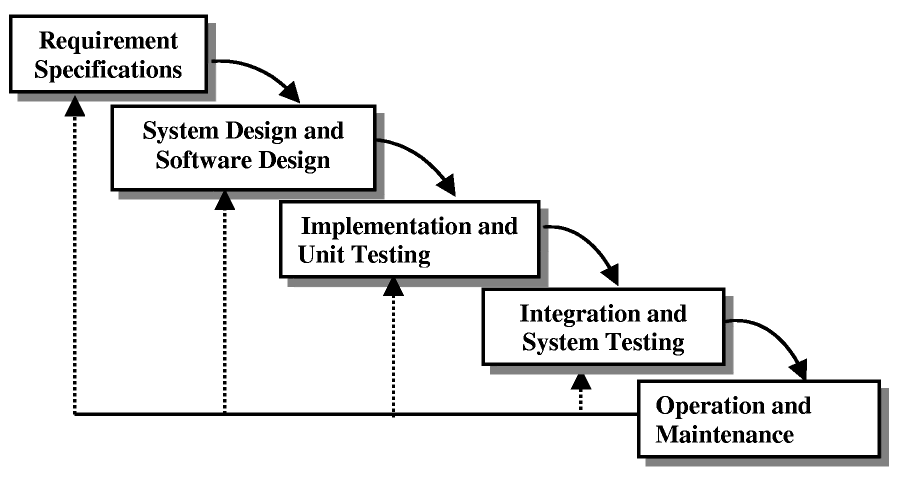
\includegraphics[width=.6\textwidth]{figures/waterfallmodel.png}
\end{figure}

A number of phases exist; requirements, design, implementation, verification, maintenance. Each phase has a clear purpose. It is necessary to be able to define the problem very precisely and in detail. A number of challenges exist:

\begin{itemize}
    \item Based only on specifications but they are difficult to produce and understand
    \item Difficult to get the users to describe their work
    \item Non-technical aspects are difficult to specify
    \item Requirements are changing over time
    \item Works only when we know exactly what we want and we are able to describe it precisely and unambiguously
    \item Feedback loops become necessary
    \item Many negative effects of the systems developed
\end{itemize}

\subsection{Iterative-model}
\begin{figure}[H]
    \centering
    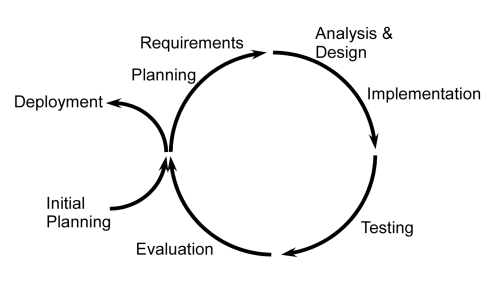
\includegraphics[width=.4\textwidth]{figures/iterativemodel.png}
\end{figure}
A model of steps that can be iterated a number of times.

\begin{itemize}
    \item Evolution with prototypes
    \item No set of clear requirements to depart from
    \item The understanding of the problem is changing during development
    \item Development through a series of cycles
    \item The requirements and the system are improved in each iteration
\end{itemize}

\subsection{Example one}
The B\&K systems were developed with a waterfall model and it involved a number of phases from requirements to release. The new project involved prototype development and some evaluation in the requirements phase, therefore some iteration was present.

\subsection{Example two}
Visualisation of blood tests results for diagnosing\footnote{Adam Viggo Glistrup and Dennis Dalgaard (2016) UI Prototypes ‐ Identification of software requirements in a highly complex domain. Master thesis, Aalborg University, Department of Computer Science.}.

Impossible for developers to learn enough about the diagnosis process to enable them to produce a prototype. The preference of doctors is an important point as well. Boundary object; physical object with different representation, drawings, illustrations, and more. Used boundary objects to facilitate discussion with the medical doctors and illustrate options.

\section{Contingency theory}
How do you intelligently choose between waterfall- and iterative-method? The relevance of these categories of methods can be determined from contingency factors. Analyse uncertainty in terms of the following four factors:

\begin{itemize}
    \item the organisational and technical context of the system
    \item the future computer system
    \item the experience and skills of the users
    \item the experience and skills of the system developers
\end{itemize}

Selection of approach; if uncertainty is low, base requirements determination of an informal approach or on analysis of existing systems, or if uncertainty is high, use specifications or prototypes. 

Furthermore; there's a distinction between complexity and uncertainty.

Uncertainty is; the degree of structuredness that characterises the users' work, the degree of understanding the users have about their work, and the degree of experience and training of the system developers.

Complexity is; the project size, number of users, volume of new information, and complexity of new information.

\begin{figure}[H]
    \centering
    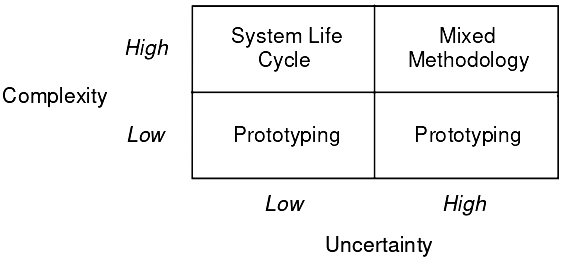
\includegraphics[width=.5\textwidth]{figures/complexityuncertaintymodel.png}
\end{figure}

\subsection{Principle of limited reduction}
Contingencies should be analysed dynamically throughout a development project. The principle of limited reduction: 

\begin{figure}[H]
    \centering
    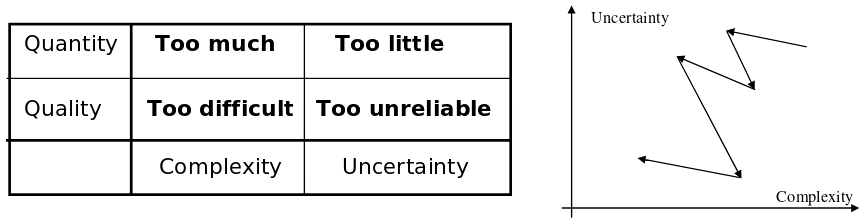
\includegraphics[width=.5\textwidth]{figures/limitedreduction.png}
\end{figure}

\begin{itemize}
    \item Relying on an analytical mode of operation \textit{to reduce complexity} introduces new sources of uncertainty requiring experimental countermeasures.
    \item Relying on an experimental mode of operation to \textit{reduce uncertainty} introduces new sources of complexity requiring analytically countermeasures.
\end{itemize}

\section{Strategy with \ad}

Top-down strategy means doing each task sequentially, almost waterfall-ish but in one stretch, executing quality assurance periodically. Similarly, \textit{use-case driven}, architecture-centric, and incremental methods iterate each prototype incrementally based on some requirement, that being user-stories, etc.

\subsection{Activities}
From existing documentation, the task is characterised, difficulties are evaluated, a strategy is formulated, which leads to an \textbf{analysis and design strategy}, which guides the object-oriented analysis and design (\ad).

\subsection{Characterise the task}
Using a checklist, asking questions on the basic characteristics of the task and the actors interacting with it, both during development and eventual use. Whichever part of the checklist that has the most uncertainty should be the focus of the strategy. Tailor the strategy to resolve these difficulties first. 

\begin{figure}[H]
    \centering
    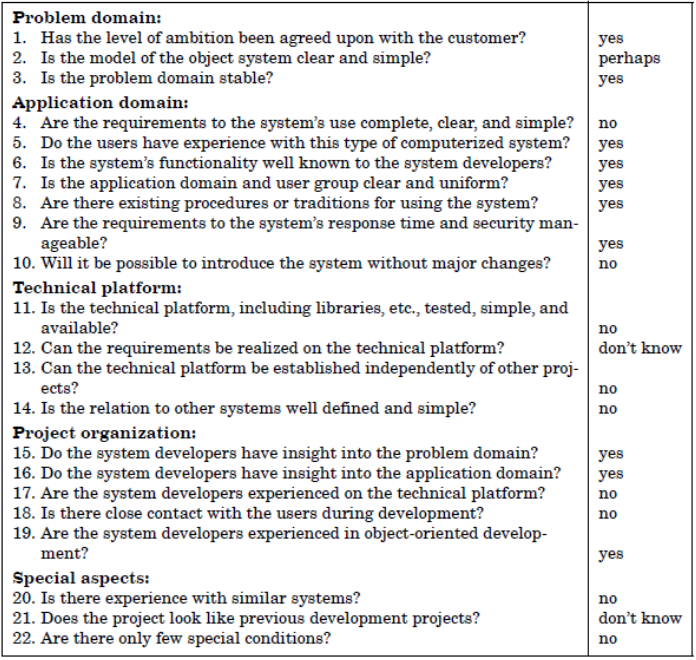
\includegraphics[width=.7\textwidth]{figures/checklist.png}
\end{figure}

\subsection{Evaluate difficulties}
Using the checklist, grade each activity on difficulty as $0$ for yes, $1$ for perhaps, and $2$ for no or unknown. This gives you an overview of the most difficult activities in the \ad-method. Then tailor the strategy to resolve the most significant difficulties first.
\begin{figure}[H]
    \centering
    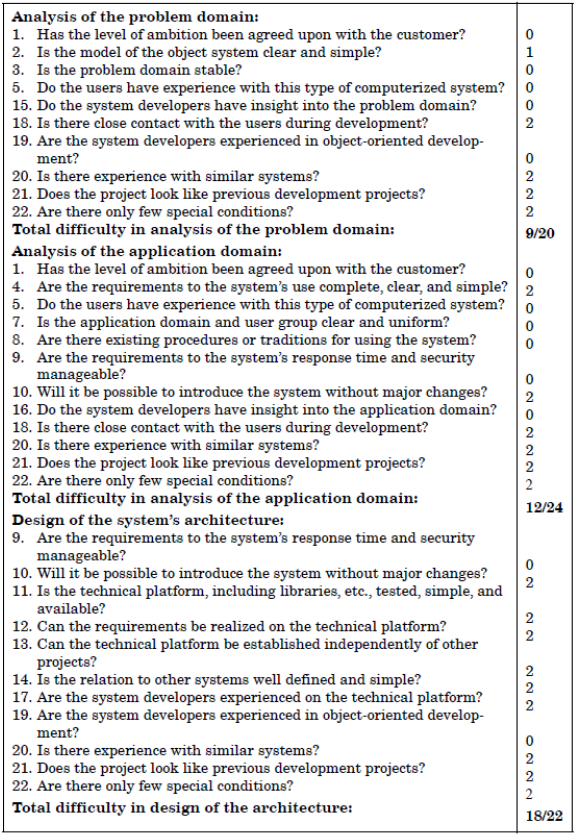
\includegraphics[width=.7\textwidth]{figures/checklistevaluatediff.png}
\end{figure}

\subsection{Summary}
\begin{figure}[H]
    \centering
    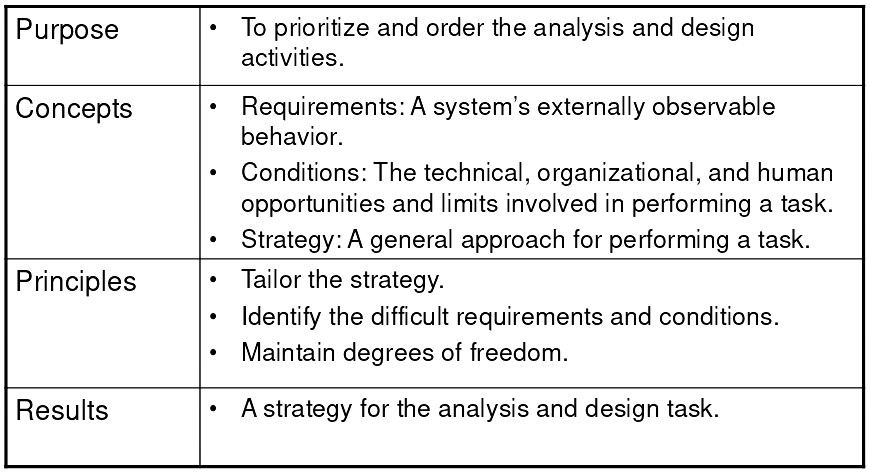
\includegraphics[width=.7\textwidth]{figures/strategysummary.png}
\end{figure}

\section{Principles}
\subsection{Tailor the strategy}
To efficiently use development resources to mange difficulties in a software project, a strategy must be tailored to the situation.

\subsection{Identify the difficult requirements and conditions}
The big project challenges and problems stem from disparity between requirements and realities. It is important that the development strategy identifies critical areas that require special effort and attention.

\subsection{Maintain degrees of freedom}
Unexpected problems will appear during analysis and design. The strategy should ensure that degrees of freedom are maintained for a possible redesign of system parts later in the process.

